\section{Instalación y despliegue de la aplicación} \label{anex:desp}

En esta sección se va a hacer una guía sobre los pasos necesarios para llevar a cabo una correcta instalación de servicios y dependencias para la aplicación \texttt{SIVIRA}.

\subsection{Instalación mínima}

Se instalarán los componentes mínimos y necesarios para que la aplicación pueda ejecutarse correctamente. Estos son:

\begin{itemize}
\item RabbitMQ.
\item SQLite3.
\item Dependencias de Python3.
\item Dependencias para el servidor de streaming.
\end{itemize}


\textbf{Servicio RabbitMQ}

RabbitMQ es un broker de mensajes de código abierto. Es necesario para poder gestionar las colas de las tareas asíncronas de la aplicación utilizadas por \texttt{celery}.

Se puede instalar fácilmente usando el siguiente comando:

\vspace{-1.4cm}

\begin{verbatim}

# sudo apt-get install rabbitmq-server

\end{verbatim}

\vspace{-1.4cm}

Por defecto, \texttt{RabbitMQ} escuchará en el puerto 5672 en todas las interfaces disponibles. Puede comprobar si el servicio está disponible con:


\vspace{-1.4cm}

\begin{verbatim}

# sudo service rabbitmq-server status

\end{verbatim}

\vspace{-1.4cm}

\textbf{SQLite3}

Para almacenar los estados de las tareas asíncronas, es necesario especificar un backend de almacenamiento. En este caso, se ha seleccionado \texttt{SQLite} ya que es muy ligero y fácil de usar y configurar.

Puede instalar fácilmente este servicio, usando el comando:

\vspace{-1.4cm}

\begin{verbatim}

# sudo apt-get install sqlite3

\end{verbatim}

\vspace{-1.4cm}

Una vez instalado, compruebe que puede acceder al terminal sqlite con el comando:

\vspace{-1.4cm}

\begin{verbatim}

# sqlite3

\end{verbatim}

\vspace{-1.4cm}

\textbf{Dependencias de Python}

Para instalar las dependencias de Python, se recomienda crear un entorno virtual. Puede crear uno rápidamente usando el comando:

\vspace{-1.4cm}

\begin{verbatim}

# python3 -m venv ./venv

\end{verbatim}

\vspace{-1.4cm}

A continuación, puede activar ese entorno utilizando:

\vspace{-1.4cm}

\begin{verbatim}

# source venv/bin/activate

\end{verbatim}

\vspace{-1.4cm}

Después, puede instalar todas las dependencias necesarias utilizando el siguiente comando:

\vspace{-1.4cm}

\begin{verbatim}

# pip3 install -r minium_requirements.txt

\end{verbatim}

\vspace{-1.4cm}

\textbf{Dependencias para el servidor de streaming}

Para la transmisión del vídeo en tiempo real, es necesario instalar el siguiente paquete de códecs para websockets.

\vspace{-1.4cm}

\begin{verbatim}

# sudo apt-get install ffmpeg python3-ws4py

\end{verbatim}

\vspace{-1.4cm}

\newpage

\subsection{Instalación completa}

La instalación completa incluye el procesamiento de imágenes para la detección de objetos utilizados por el agente detector de objetos, cuya funcionalidad es filtrar las alertas generadas por el agente de movimiento, alertando sólo en el caso de detectar a una persona en la imagen capturada durante la alerta.


\begin{tabular}{|p{15.5cm}|}
	
	\hline
	
	\textit{ \textbf{*Nota:} Antes de iniciar esta instalación, es necesario haber realizado la instalación requerida descrita en el apartado anterior. }
	\\
	\hline
	
\end{tabular}

Esta instalación es opcional, ya que puede desactivar esta funcionalidad estableciendo el valor a \texttt{False} en la opción \texttt{DETECTOR\_AGENT\_STATUS} en el archivo de configuración \texttt{settings.py}.

En esta instalación se instalarán los siguientes componentes:

\vspace{-0.5cm}

\begin{itemize}
\item Tensorflow.
\item OpenCV.
\item Protobuf.
\item Dependencias de Python.
\end{itemize}
    
\textbf{Tensorflow}

\texttt{Tensorflow} es un framework que se utilizará para el reconocimiento de objetos en imágenes. Para su instalación, podemos utilizar el siguiente comando:

\vspace{-1.4cm}

\begin{verbatim}

# pip3 install Tensorflow==1.14.0

\end{verbatim}

\vspace{-1.4cm}

O instale las dependencias incluidas en el archivo \texttt{full\_requirements.txt}, donde se instalarán los paquetes \texttt{Tensorflow} para Python.

\vspace{-1.4cm}

\begin{verbatim}

# pip3 install -r full_requirements.txt

\end{verbatim}

\vspace{-1cm}

\begin{tabular}{|p{15.5cm}|}
	
	\hline
	
	\textit{\textbf{Advertencia}: Es posible que si todas las bibliotecas se instalan desde el archivo \texttt{full\_requirements.txt}, se produzca un fallo de memoria, debido al hecho de que estas bibliotecas son muy pesadas y se almacenan en la caché cuando se descargan (antes de ser instaladas). Si se produce este error, simplemente instale el paquete \texttt{Tensorflow} manualmente, como se indica al principio.}
	\\
	\hline
	
\end{tabular}

A continuación, es necesario ejecutar los siguientes comandos para instalar algunas dependencias necesarias para \texttt{Tensorflow}.

\vspace{-1.4cm}

\begin{verbatim}

# sudo apt-get install libatlas-base-dev
# sudo pip3 install pillow lxml matplotlib cython
# sudo apt-get install python-tk

\end{verbatim}

\vspace{-1.4cm}

\textbf{OpenCV}

Los ejemplos de detección de objetos de \texttt{Tensorflow} normalmente utilizan matplotlib para mostrar imágenes, pero es preferible usar \texttt{OpenCV} porque es más fácil para trabajar y menos propenso a errores.

Para que \texttt{OpenCV} funcione en la Raspberry Pi, hay bastantes dependencias que necesitan ser instaladas a través de `apt-get'. Si alguno de los siguientes comandos no funciona, entonces ejecute el comando `sudo apt-get update' e inténtelo de nuevo.


\vspace{-1.4cm}

\begin{verbatim}

# sudo apt-get install libjpeg-dev libtiff5-dev libjasper-dev libpng12-dev
# sudo apt-get install libavcodec-dev libavformat-dev libswscale-dev libv4l-dev
# sudo apt-get install libxvidcore-dev libx264-dev
# sudo apt-get install qt4-dev-tools

\end{verbatim}

\vspace{-1.4cm}

Ahora que tenemos todas estas dependencias instaladas, podemos instalar \texttt{OpenCV}, usando:


\vspace{-1.4cm}

\begin{verbatim}

# pip3 install opencv-python

\end{verbatim}

\vspace{-1.4cm}

O puede utilizar al archivo que contiene las dependencias necesarias:

\vspace{-1.4cm}

\begin{verbatim}

# pip3 install -r full_requirements.txt

\end{verbatim}

\vspace{-1.4cm}

\newpage

\textbf{Compilar e instalar Protobuf}

La API de detección de objetos de \texttt{TensorFlow} utiliza \texttt{Protobuf}, un paquete que implementa el formato de datos \texttt{Protocol Buffer} de Google. Desafortunadamente, actualmente no hay una manera fácil de instalar el \texttt{Protobuf} en la Raspberry Pi. Tenemos que compilarlo desde el código fuente nosotros mismos y luego instalarlo.

Primero, obtenga los paquetes necesarios para compilar \texttt{Protobuf} desde el código fuente:

\vspace{-1.4cm}

\begin{verbatim}

# sudo apt-get install autoconf automake libtool curl

\end{verbatim}

\vspace{-1.4cm}

A continuación, descargue la versión \texttt{Protobuf} del repositorio GitHub:

\vspace{-1.4cm}

\begin{verbatim}

# wget https://github.com/protocolbuffers/protobuf/releases/download/v3.9.0/
protobuf-all-3.9.0.tar.gz

\end{verbatim}

\vspace{-1.4cm}

Si hay una versión más reciente de protobuf disponible, descárguela en su lugar. Descomprima el archivo y situése en la carpeta:

\vspace{-0.5cm}

\begin{verbatim}
# tar -zxvf protobuf-all-3.9.0.tar.gz
# cd protobuf-3.9.0
\end{verbatim}

\vspace{-0.5cm}

Configure la compilación ejecutando el siguiente comando (tarda alrededor de unos 2 minutos):

\vspace{-0.7cm}

\begin{verbatim}
# ./configure
\end{verbatim}

\vspace{-0.5cm}

Construya el paquete (Este proceso tarda alrededor de unos 61 minutos):

\vspace{-0.8cm}

\begin{verbatim}
# make
\end{verbatim}

\vspace{-0.5cm}

A continuación ejecute (Este proceso tarda alrededor de unos 108 minutos):

\vspace{-0.8cm}

\begin{verbatim}
# make check 
\end{verbatim}

\vspace{-0.5cm}

Según otras guías que he visto, este comando puede salir con errores, pero \texttt{Protobuf} seguirá funcionando. Si ve errores, puede ignorarlos por ahora. Ahora que está construido, instálelo:

\vspace{-0.8cm}

\begin{verbatim}
# sudo make install
\end{verbatim}

\vspace{-0.5cm}

A continuación, muévase al directorio Python y exporte la ruta de la biblioteca:

\vspace{-0.8cm}

\begin{verbatim}
# cd python
# export LD_LIBRARY_PATH=../src/.libs
\end{verbatim}

\vspace{-0.5cm}

\newpage

A continuación ejecute:

\vspace{-0.8cm}

\begin{verbatim}
# python3 setup.py build --cpp_implementation 
# python3 setup.py test --cpp_implementation
# sudo python3 setup.py install --cpp_implementation
\end{verbatim}

\vspace{-0.5cm}

A continuación, ejecute los siguientes comandos:

\vspace{-0.8cm}

\begin{verbatim}
# export PROTOCOL_BUFFERS_PYTHON_IMPLEMENTATION=cpp
# export PROTOCOL_BUFFERS_PYTHON_IMPLEMENTATION_VERSION=3
\end{verbatim}

\vspace{-0.5cm}

Finalmente, ejecute:

\vspace{-0.8cm}

\begin{verbatim}
# sudo ldconfig
\end{verbatim}

\vspace{-0.5cm}

¡Eso es todo! Ahora \texttt{Protobuf} está instalado en la Raspberry PI. Comprueba que está instalado correctamente ejecutando el siguiente comando y asegurándote de que muestra el texto de ayuda predeterminado.

\vspace{-0.8cm}

\begin{verbatim}
# protoc
\end{verbatim}

\vspace{-0.5cm}

Por alguna razón, es necesario reiniciar después de este proceso:

\vspace{-0.8cm}

\begin{verbatim}
# sudo reboot now
\end{verbatim}

\vspace{-0.5cm}

Una vez completado este paso, la instalación se ha completado.

\subsection{Despliegue de la aplicación}

En esta sección veremos cómo podemos configurar y desplegar la aplicación.

Los pasos para desplegar la aplicación son los siguientes:

\vspace{-0.4cm}

\begin{itemize}
\item Crear el bot de Telegram
\item Descargar el proyecto del repositorio de Github.
\item Configurar la aplicación.
\item Ejecutar la aplicación.
\end{itemize}

\newpage

\textbf{Crear el bot de Telegram}

Telegrama es un servicio de mensajería instantánea y voz sobre IP basado en la nube. La aplicación de Telegram es multiplataforma.

\vspace{-0.4cm}

\begin{itemize}

\item En primer lugar, descargue la aplicación, instálela y regístrese con su número de móvil. Luego, debe buscar el nombre de \texttt{BotFather} en el motor de búsqueda.

\begin{figure}[h]
	\centering
	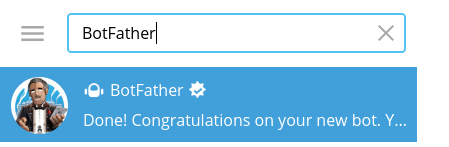
\includegraphics[scale=0.6]{images/57}
	\caption{Búsqueda de BothFather en Telegram}
\end{figure}

\item Por último, debe iniciar una conversación con este bot para poder crear su propio bot. Para ello, puede utilizar el comando \texttt{/newbot} para comenzar el proceso de creación del bot. Es muy simple y rápido. A continuación se muestra un ejemplo.


\begin{figure}[h]
	\centering
	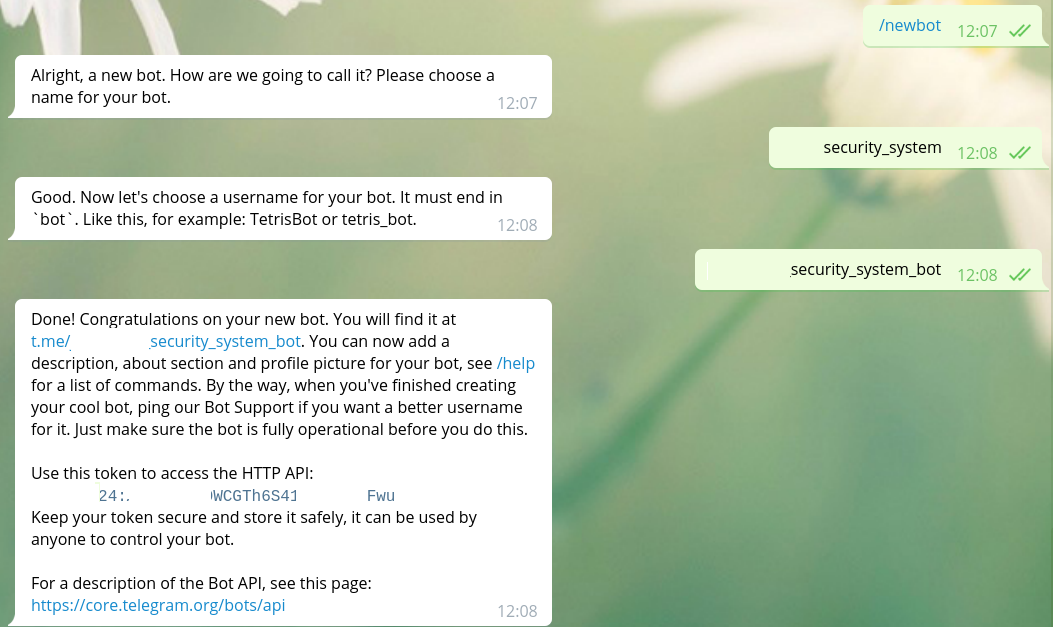
\includegraphics[scale=0.45]{images/58}
	\caption{Búsqueda de BothFather en Telegram}
\end{figure}

\end{itemize}

\begin{tabular}{|p{15.5cm}|}
	
	\hline
	
	\textit{\textbf{Nota:} Una vez creado el bot, es muy importante que guarde el \texttt{API token}, ya que es necesario insertarlo en la configuración que se realizará más adelante.}
	\\
	\hline
	
\end{tabular}

\newpage

\textbf{Descargue el proyecto del repositorio de Github}

El repositorio contiene todo el código fuente que necesitará para construir y ejecutar la aplicación.

Puedes descargarlo y descomprimirlo fácilmente usando la herramienta \texttt{git}.

\vspace{-0.8cm}

\begin{verbatim}
# git clone https://github.com/jmv74211/TFM_security_system_PI.git | tar -xzvf 
\end{verbatim}

\vspace{-0.5cm}

\begin{tabular}{|p{15.5cm}|}
	
	\hline
	
	\textit{\textbf{Nota}: Si no tiene la herramienta git instalada, puede acceder a la \href{https://github.com/jmv74211/TFM_security_system_PI}{página del repositorio} y descargarla con un archivo zip.}
	\\
	\hline
	
\end{tabular}

\textbf{Configure la aplicación}

Para modificar los archivos de configuración es necesario dirigirse al directorio \texttt{config} dentro de \texttt{src}.

\begin{itemize}

\item Primero, vamos a \textbf{generar un hash para la contraseña} de la \texttt{API}. Para ello, utilizaremos la utilidad \href{https://github.com/jmv74211/TFM_security_system_PI/blob/master/src/tools/generate_hash_password.py}{generate\_hash\_password.py} que se encuentra dentro del directorio de \href{https://github.com/jmv74211/TFM_security_system_PI/tree/master/src/tools}{tools}.

Para obtener el hash de la contraseña:

\vspace{-0.5cm}

\begin{verbatim}
$ python3 generate_hash_password.py 
Enter your password: password_test
Your hash password is  sha256$hqhX2BpC$638ce4...

\end{verbatim}

\vspace{-0.5cm}

\item A continuación, necesitamos introducir las \textbf{credenciales de inicio de sesión} para nuestra \texttt{API}. Vaya al archivo \href{https://github.com/jmv74211/TFM_security_system_PI/blob/master/src/config/authentication.yml}{authentication.yml} y establezca las credenciales de acceso para la \texttt{API} de la aplicación (tiene que añadir el hash de usuario y contraseña que se ha obtenido en el paso anterior).

\item El siguiente paso es \textbf{configurar las credenciales del Telegram}. Para ello, debe editar el archivo \href{https://github.com/jmv74211/TFM\_security\_system\_PI/blob/master/src/config/telegram\_config.yml}{telegram\_config.yml} y añadir la información que se solicita en la plantilla.

\begin{tabular}{|p{15.5cm}|}
	
	\hline
	
	\textit{\textbf{Nota}: Si no conoce todos los datos, no se preocupe, pueden obtenerse más tarde. Los datos obligatorios son \texttt{api\_token}, \texttt{api\_agent\_user} y \texttt{api\_agent\_password}. (Tenga en cuenta que en este caso es necesario introducir la contraseña en formato crudo, (sin cifrar).}
	\\
	\hline
	
\end{tabular}

\item Si ha realizado una instalación completa (instalado los componentes necesarios para el agente detector de objetos), entonces tiene que establecer el valor de la variable \texttt{OBJECT\_DETECTOR\_INSTALLED} a `True' en \href{https://github.com/jmv74211/TFM_security_system_PI/blob/master/app.sh}{app.sh} para poder iniciar el agente de detección de objetos al ejecutar la aplicación.

\item El último paso del proceso de configuración es modificar el archivo de configuración \href{https://github.com/jmv74211/TFM_security_system_PI/blob/master/src/settings.py}{settings.py}. En este fichero podemos modificar la configuración general de la aplicación, como direcciones IP de servicios, puertos....

La configuración mínima necesaria es la siguiente:

\begin{itemize}
\item \textbf{API\_AGENT\_IP\_ADDRESS}: Dirección IP de Raspberry PU que está ejecutando el servicio de la \texttt{API}. Si la instalación es local, introduzca la dirección IP local. Ejemplo: \textit{192.168.1.100}.
\item \textbf{API\_PASSWORD}: Su contraseña en crudo del agente de la API (sin encriptar). Ejemplo: \textit{"prueba"}
\item \textbf{GPIO\_SENSOR\_PIN\_NUMBER}: El número de pin del sensor GPIO donde se ha conectado el sensor de movimiento. Si ha seguido la instalación de hardware anterior, entonces será el número 16. Tenga en cuenta que el modo de numeración es \texttt{GPIO.BOARD}.   
\item \textbf{STREAMING\_SERVER\_IP\_ADDRESS}: Dirección IP de la Raspberry PI que está ejecutando el servicio de streaming. Si la instalación es local, introduzca la dirección IP local. \textit{192.168.1.100}.    
\item \textbf{DETECTOR\_AGENT\_IP\_ADDRESS}: Dirección IP de la Raspberry PI que está ejecutando el servicio de detección de objetos. Si la instalación es local, introduzca la dirección IP local. \textit{192.168.1.100}.
 
\end{itemize}

\begin{tabular}{|p{15.5cm}|}
	
	\hline
	
	\textit{\textbf{Advertencia}: Tenga cuidado con la sintaxis y la información que va a modificar. Cualquier error en los archivos de configuración hará que la aplicación no funcione correctamente.}
	\\
	\hline
	
\end{tabular}

\end{itemize}

\newpage

\textbf{Ejecuta la aplicación}

Una vez que la aplicación está instalada y configurada, podemos ejecutarla usando el script \href{https://github.com/jmv74211/TFM_security_system_PI/blob/master/app.sh}{app.sh} ubicado en el directorio raíz de la aplicación.

\vspace{0.3cm}

\begin{tabular}{|p{15.5cm}|}
	
	\hline
	
	\textit{\textbf{Nota}: Recuerde que si ha realizado una instalación completa (componentes necesarios para el agente detector de objetos) debe establecer el valor de la variable  \texttt{OBJECT\_DETECTOR\_INSTALLED} a `True' en app.sh para poder iniciar todos los servicios.}
	\\
	\hline
	
\end{tabular}


\begin{itemize}

\item En primer lugar, hay que darle permisos de ejecución para utilizar el script.

\vspace{-0.5cm}

\begin{verbatim}
$ sudo chmod u+x ./app.sh
\end{verbatim}

\vspace{-0.5cm}

\item Para iniciar la aplicación, ejecute el comando:

\vspace{-0.5cm}

\begin{verbatim}
$ ./app.sh start
\end{verbatim}

\vspace{-0.5cm}

\item Para parar la aplicación, ejecute el comando:

\vspace{-0.5cm}

\begin{verbatim}
$ ./app.sh stop
\end{verbatim}

\vspace{-0.5cm}

\item Para comprobar el estado de la aplicación, ejecute el comando:

\vspace{-0.5cm}

\begin{verbatim}
$ ./app.sh status
\end{verbatim}

\vspace{-0.3cm}


\end{itemize}

\begin{tabular}{|p{15.5cm}|}
	
	\hline
	
	\textit{\textbf{Atención:} Si no ha configurado las credenciales de Telegram (nombre de usuario de Telegram, ID, nombre de usuario e ID del bot) sólo podrá acceder a la sección \texttt{utils} del bot para obtener estas credenciales. Una vez obtenidas, añádalas al archivo de configuración y reinicie la aplicación (stop and start).
	}
	\\
	\hline
	
\end{tabular}





